\documentclass[10pt,twocolumn]{article}

\usepackage[a4paper,margin=1.8cm]{geometry}
\usepackage{graphicx}
\usepackage{amsmath,amssymb}
\usepackage{booktabs}
\usepackage{bm}
\usepackage{float}
\usepackage{caption}
\usepackage{subcaption}
\usepackage{xcolor}
\usepackage{hyperref}
\usepackage{enumitem}
\usepackage{microtype}

\hypersetup{
    colorlinks=true,
    linkcolor=blue,
    citecolor=blue,
    urlcolor=blue
}

\setlength{\columnsep}{0.7cm}

\title{
    \textbf{
        Experimental Observations on the
        Statistical Mechanics of a Chronically Late
        Theoretical Physicist
    }
}

\author{
    Anonymous Observer \\
    Department of Temporal Dynamics \\
    Institute for Advanced Scheduling Failures
}

\date{August 2026}

\begin{document}

\twocolumn[
\maketitle
\vspace{-1.2cm}

\begin{abstract}
We present a longitudinal observational study of the punctuality
behavior of a theoretical physicist over a fourteen-week academic
window (14~April -- 24~July 2026).
A total of $N=61$ scheduled events were recorded, of which $39$
were attended and $22$ were no-shows, corresponding to a detector
inefficiency of $36\%$.
Conditional on attendance, the arrival-time residual has mean
$\mu=13.3$~min, median $12$~min, and standard deviation
$\sigma=12.8$~min.
The empirical punctuality rate, defined strictly as
$\Delta t\le 0$, is only $15\%$.
The delay distribution is positively skewed, poorly described by a
single Gaussian, and consistent with an exponential late-time tail
of scale $\tau\simeq 15$~min.
Event type, weekday, and scheduled hour act as relevant operators:
functional-analysis lectures at noon remain a strongly coupled
sector, whereas Friday Mathematica exercises stay comparatively
perturbative.
A single early-arrival event ($\Delta t=-3$~min) occurred under
rain on 6~May 2026 and is interpreted, with due caution, as a
candidate rain-resonance of the motivational wavefunction.
The global delay record is now $43$~min, set in a
functional-analysis lecture, thereby overtaking the barbecue.
\end{abstract}

\vspace{0.5cm}
]

\tableofcontents

\vspace{0.4cm}

% -------------------------------------------------
\section{Introduction}
% -------------------------------------------------

Punctuality is frequently modeled as a stochastic process with
approximately Gaussian fluctuations around a scheduled arrival time
$t_0$. In equilibrium statistical mechanics this would correspond
to a quadratic effective potential for the residual
\begin{equation}
    \Delta t \equiv t-t_0,
\end{equation}
with positive $\Delta t$ denoting lateness. The associated
picture is comforting: most arrivals cluster near $t_0$, large
deviations are exponentially rare, and the Central Limit Theorem
is left in peace.

Preliminary field observations of the present subject indicated
that this picture is not merely incomplete but actively misleading.
Large positive residuals, intermittent vacuum-to-absent transitions,
and a near-total absence of early arrivals suggest dynamics beyond
the perturbative Gaussian regime. In the language of this paper,
the subject does not fluctuate around punctuality; punctuality
fluctuates, weakly, around the subject.

The scientific objectives are threefold.
First, we characterize the one-point statistics of $\Delta t$
and the no-show probability.
Second, we test whether the delay distribution admits a simple
parametric description --- a Gaussian core, an exponential tail,
or a mixture of both.
Third, we search for correlations with environmental and academic
covariates: weather, temperature, event type, weekday, and time of
day.

A working hypothesis, to be confronted with the data, is that
lateness is an effective coupling $g$ that runs with the
\textit{energy scale} of the appointment. Lectures, especially those
in functional analysis, are expected to lie in a strongly coupled
phase. Meetings, exercises, and lunches may remain closer to the
Gaussian fixed point. Social events (here, a single barbecue)
provide a useful out-of-sample check: if the coupling is universal,
the barbecue should be late as well.

% -------------------------------------------------
\section{Experimental Setup}
% -------------------------------------------------

Data were acquired by direct observation between 14~April and
24~July 2026, a window of $101$ days. For each scheduled event
the nominal time $t_0$ and, when applicable, the observed arrival
time $t$ were recorded to the nearest minute. The catalog
comprises $N=61$ events.

Measured observables included:
\begin{itemize}[leftmargin=0.4cm]
    \item event category
          (lecture, exercise, meeting, lunch, barbecue),
    \item academic subject
          (functional analysis, Mathematica, project management,
          mensa),
    \item weather conditions and ambient temperature,
    \item weekday and scheduled hour,
    \item attendance state (attended / absent).
\end{itemize}

No-show events are treated as detector inefficiencies rather than
as $\Delta t\to+\infty$. They are excluded from fits to the delay
distribution but retained in the computation of the absence
probability. Two late-June absences are tagged \texttt{Berlin}
in the log and correspond to a documented off-site period of the
detector; they are kept in the absence sample, since an empty
chair is an empty chair.

The operational definition of punctuality adopted throughout is
strict,
\begin{equation}
    \text{punctual} \;\Longleftrightarrow\; \Delta t \le 0.
\end{equation}
A five-minute grace window, while socially widespread, would
constitute an unacceptably generous infrared cutoff and is not
used.

The sample remains modest by the standards of a thermodynamic
limit. Several subgroups (rain, drizzle, barbecue) still contain
a single point. All such statements below should be read as
phenomenological rather than as claims of asymptotic significance.
The subject remained unaware of the experiment during data
acquisition, which we take as a reasonable guarantee against
observer-induced collapse of the motivational wavefunction.

\subsection*{Experimental Data}

The experimental data can be acquired as an open dataset from \href{https://github.com/kathamatician/chronostatistics}{github}.

% -------------------------------------------------
\section{Statistical Analysis}
% -------------------------------------------------

\subsection{Core Estimators}

Let $\{\Delta t_i\}_{i=1}^{N_{\mathrm{att}}}$ denote the
$N_{\mathrm{att}}=39$ attended residuals. The sample mean and
unbiased variance are
\begin{equation}
    \mu =
    \frac{1}{N_{\mathrm{att}}}
    \sum_{i=1}^{N_{\mathrm{att}}} \Delta t_i,
    \qquad
    \sigma^2 =
    \frac{1}{N_{\mathrm{att}}-1}
    \sum_{i=1}^{N_{\mathrm{att}}}
    (\Delta t_i - \mu)^2.
\end{equation}
The measured values are
\begin{equation}
    \mu = 13.3~\mathrm{min},
    \qquad
    \sigma = 12.8~\mathrm{min},
    \qquad
    \mathrm{median} = 12~\mathrm{min}.
\end{equation}
The distribution ranges from $\Delta t=-3$~min to
$\Delta t=43$~min and has sample skewness $+0.88$.
Only six events satisfy $\Delta t\le 0$ (five exact on-time
arrivals and one early arrival), so the empirical punctuality
rate is
\begin{equation}
    P(\Delta t\le 0)
    = \frac{6}{39} \simeq 15\%.
\end{equation}
The complementary late-arrival probability among attendees is
therefore $85\%$. Independently, the no-show probability over
the full catalog is
\begin{equation}
    P_{\mathrm{absent}} = \frac{22}{61} \simeq 36\%.
\end{equation}
Taken together, the probability that the subject both appears
\emph{and} is not late is $6/61\simeq 10\%$. This is the closest
the dataset comes to a rare-event process.

\begin{table}[H]
\centering
\caption{One-point statistics of arrival-time residuals.
Delays are computed on attended events only.
Punctuality is $\Delta t\le 0$.}
\label{tab:core}
\small
\begin{tabular}{lc}
\toprule
Quantity & Value \\
\midrule
Scheduled events $N$ & 61 \\
Attended / absent & 39 / 22 \\
No-show probability & $36\%$ \\
Mean delay $\mu$ & $13.3$~min \\
Median delay & $12$~min \\
Std.\ deviation $\sigma$ & $12.8$~min \\
Skewness & $+0.88$ \\
Min / max & $-3$~min / $43$~min \\
Punctuality rate & $15\%$ \\
$P(\Delta t>0\mid\mathrm{attended})$ & $85\%$ \\
$P(\text{present and not late})$ & $10\%$ \\
\bottomrule
\end{tabular}
\end{table}

\subsection{Gaussian Core}

A maximum-likelihood Gaussian fit to the attended sample yields
$(\mu,\sigma)\simeq(13.3,12.6)$~min
(Figs.~\ref{fig:histogram}).

The Gaussian description fails in two structurally important
ways. First, it assigns appreciable probability to early arrivals
that are almost never observed: the left tail is a desert, not a
mirror of the right. Second, it underrepresents the far-late
events at $38$, $41$ and $43$~min. A quadratic potential around
$t_0$ is therefore at best an effective theory for the bulk, and
even there the peak of the histogram sits several minutes to the
left of $\mu$.

\begin{figure}[H]
    \centering
    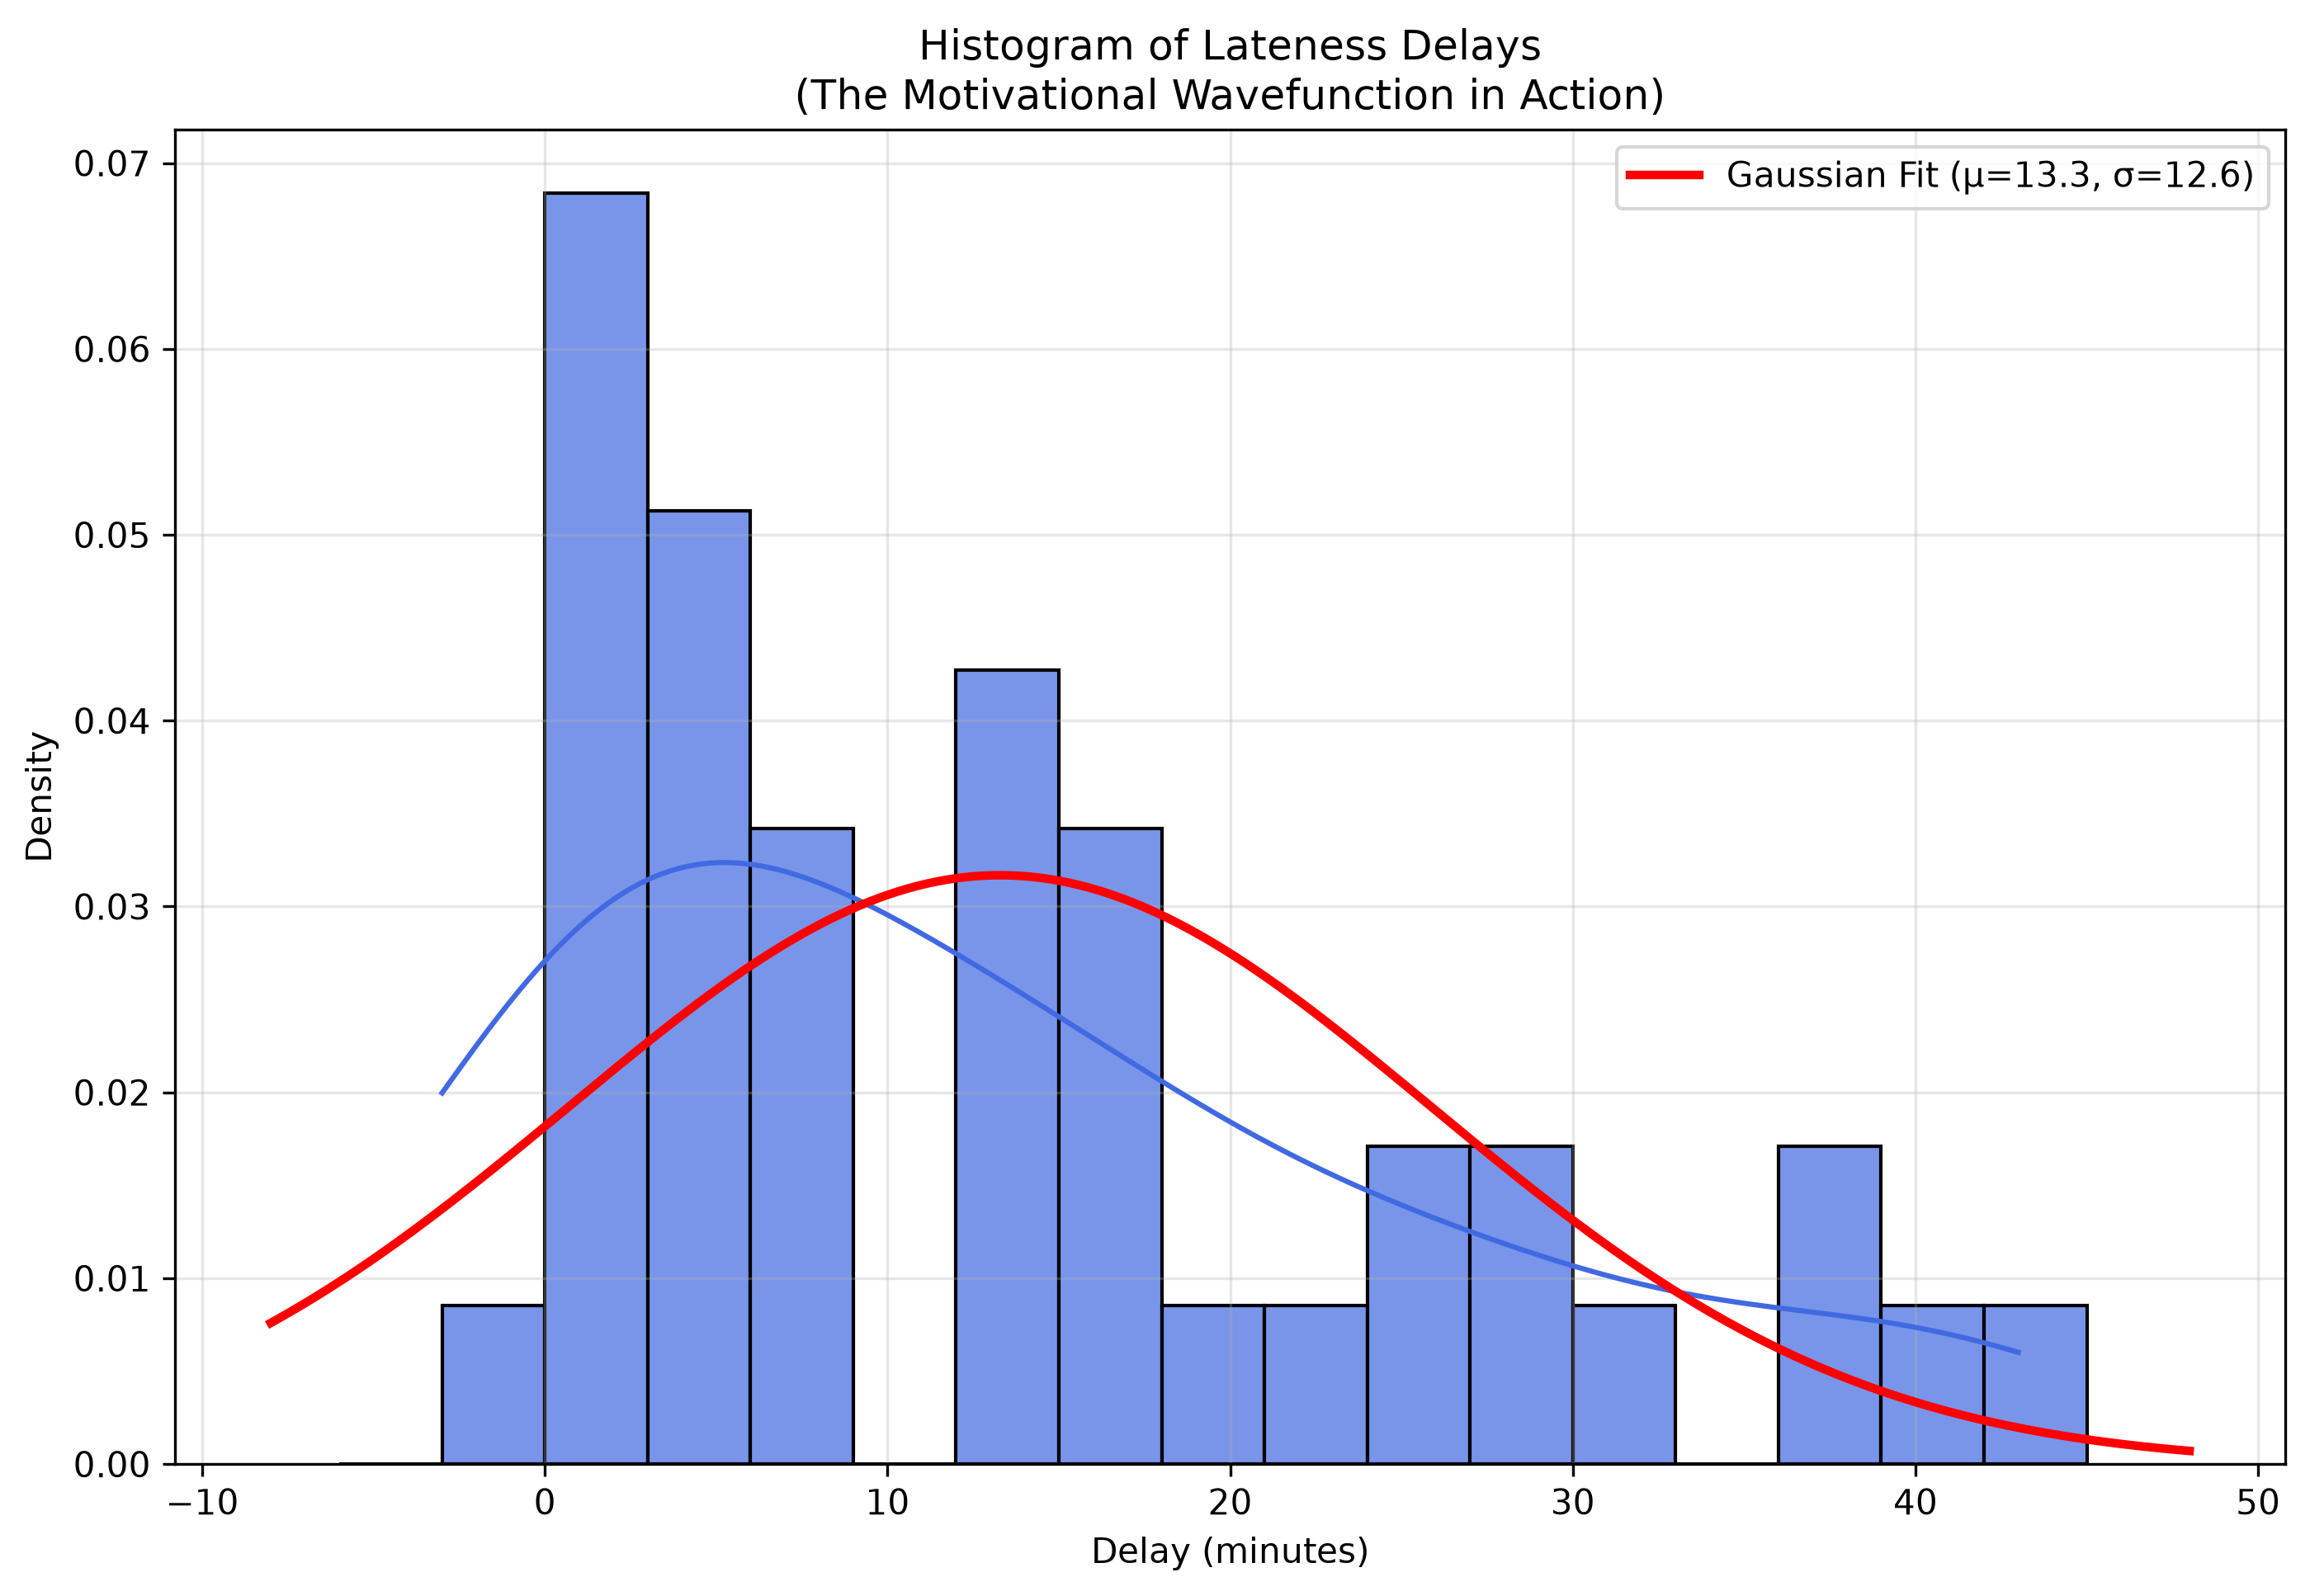
\includegraphics[width=\linewidth]{../plots/delay_histogram.png}
    \caption{
        Histogram of attended arrival-time residuals with a
        Gaussian overlay. The motivational wavefunction is
        peaked at small positive delay and leaks into a
        late-time tail. The thin blue curve is a kernel
        density estimate; it already hints that the Gaussian
        is not the right infrared theory.
    }
    \label{fig:histogram}
\end{figure}

\subsection{Exponential Tail}

Restricting to strictly positive delays ($n=33$), an exponential
model
\begin{equation}
    p(\Delta t\mid \Delta t>0)
    = \frac{1}{\tau}\,
      e^{-(\Delta t-\Delta t_{\min})/\tau}
\end{equation}
gives a fitted scale $\tau\simeq 14.8$~min
(Fig.~\ref{fig:tail}), comparable to the mean of the positive
subsample ($15.8$~min). In this description,
lateness is memoryless: conditional on not having arrived by
time $t_0+t$, the expected additional wait is still of order a
quarter of an hour. This is the statistical signature of a
process with no restoring force toward $t_0$ once the
punctuality well has been left.

\begin{figure}[H]
    \centering
    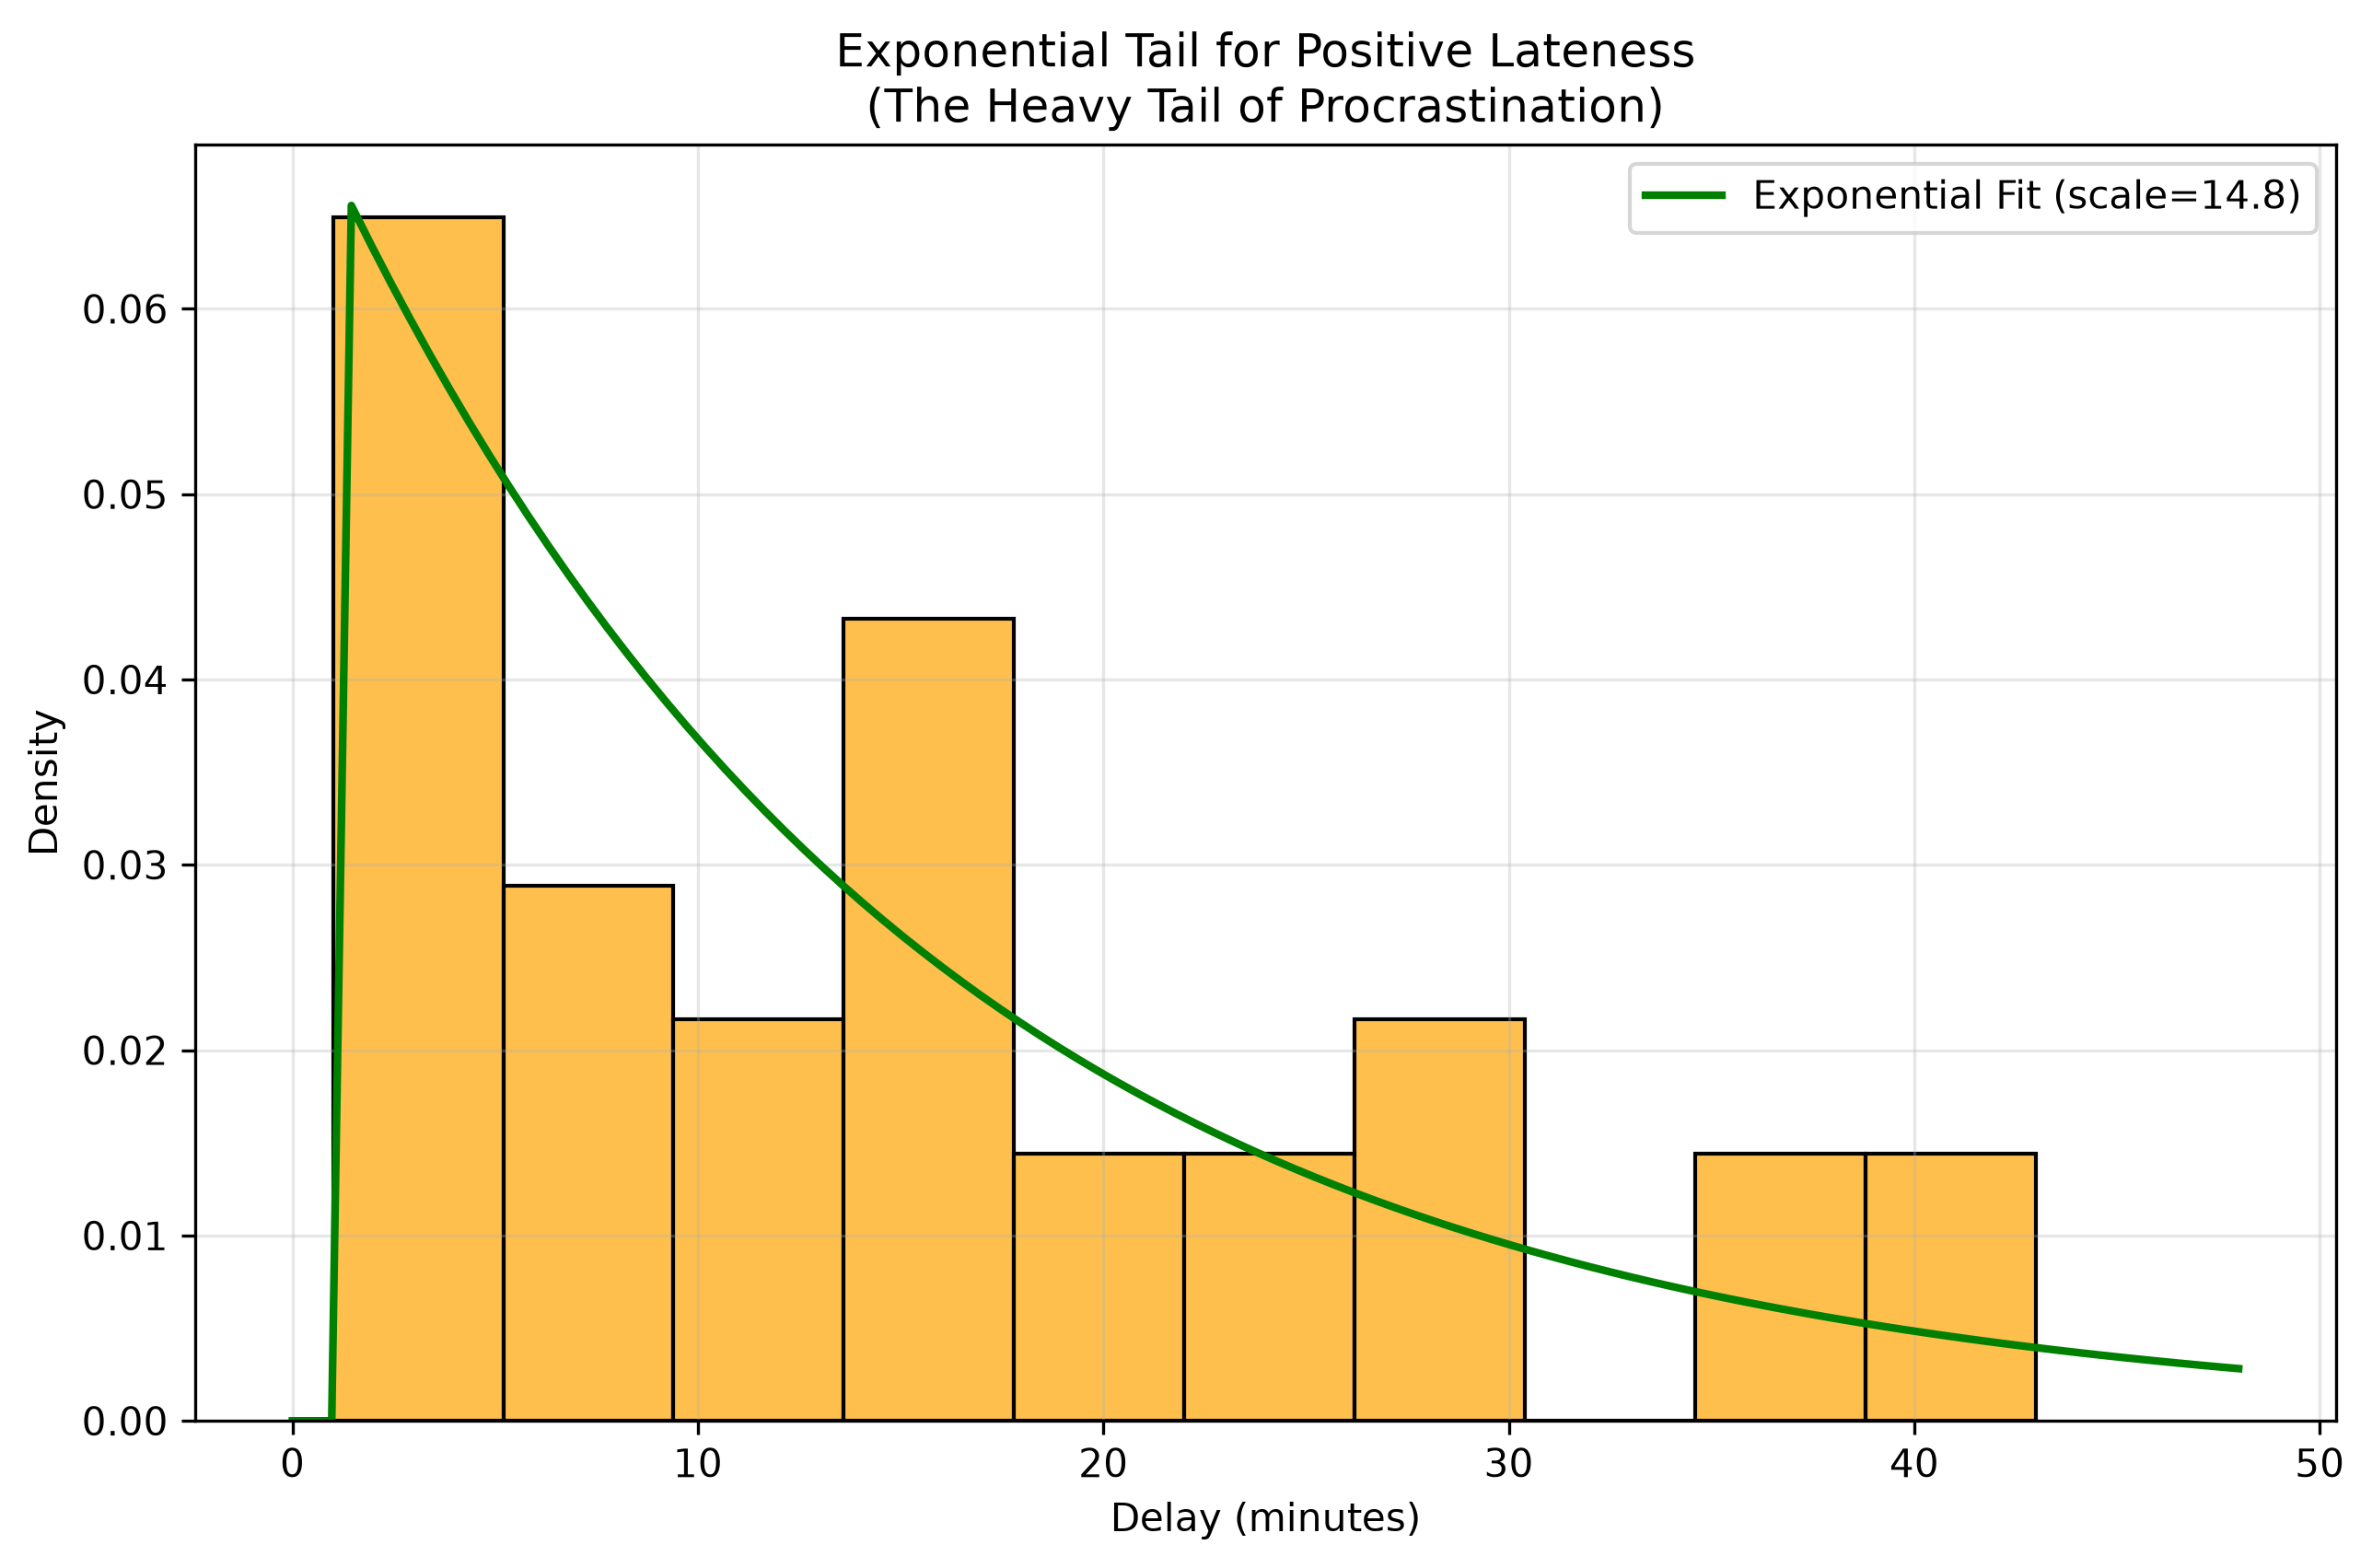
\includegraphics[width=\linewidth]{../plots/exponential_tail.png}
    \caption{
        Positive-delay subsample and exponential fit
        (scale $\tau=14.8$~min).
        The heavy tail of procrastination is, to a first
        approximation, a Poisson process in disguise.
        The scale did not run between the first and second
        observing seasons.
    }
    \label{fig:tail}
\end{figure}

A compact phenomenological model is therefore a two-regime
mixture: a narrow component supported on $\Delta t\simeq 0$
(the metastable punctuality vacuum) plus an exponential
continuum for $\Delta t>0$ (the late-time phase).
The Gaussian is the wrong interpolation between them.

\subsection{Event Type as a Relevant Operator}

Figure~\ref{fig:box} and Table~\ref{tab:event} resolve the
sample by event category. Lectures dominate both the mean
($17.8$~min) and the width of the late tail.
The effect is not uniform across subjects: attended
functional-analysis lectures average $21.3$~min ($n=10$),
while attended Mathematica lectures average $13.4$~min
($n=8$). The Mathematica sector, previously almost
perturbative, acquired a $38$~min event on 6~July and is
no longer a clean control sample. Functional analysis
remains the relevant operator.

Exercises are milder as a class (mean $8.3$~min, median
$4$~min), but the average conceals a split:
Mathematica exercises ($n=9$) sit at $5.2$~min, whereas
the three attended functional-analysis exercises average
$17.3$~min and include both the unique early arrival and
two $\sim 28$~min outliers associated with a second
observer (\textit{Simon}). Meetings remain in a comparatively
perturbative phase (mean $7.0$~min). Lunches are tightly
clustered. The barbecue produced $41$~min and held the
global record until 7~July, when a functional-analysis
lecture reached $43$~min. Universality, if it exists,
does not spare grilled food, and it does not spare
functional analysis either.

Absence rates follow a similar hierarchy: $16/34\simeq 47\%$
of lectures and $6/18=33\%$ of exercises were no-shows,
whereas every recorded meeting and lunch was attended.
Functional-analysis lectures alone are absent
$13/23\simeq 57\%$ of the time; the associated exercises
are absent $6/9=67\%$ of the time. The no-show channel
and the late-arrival channel are therefore aligned, and
both prefer the same subject.

\begin{figure}[H]
    \centering
    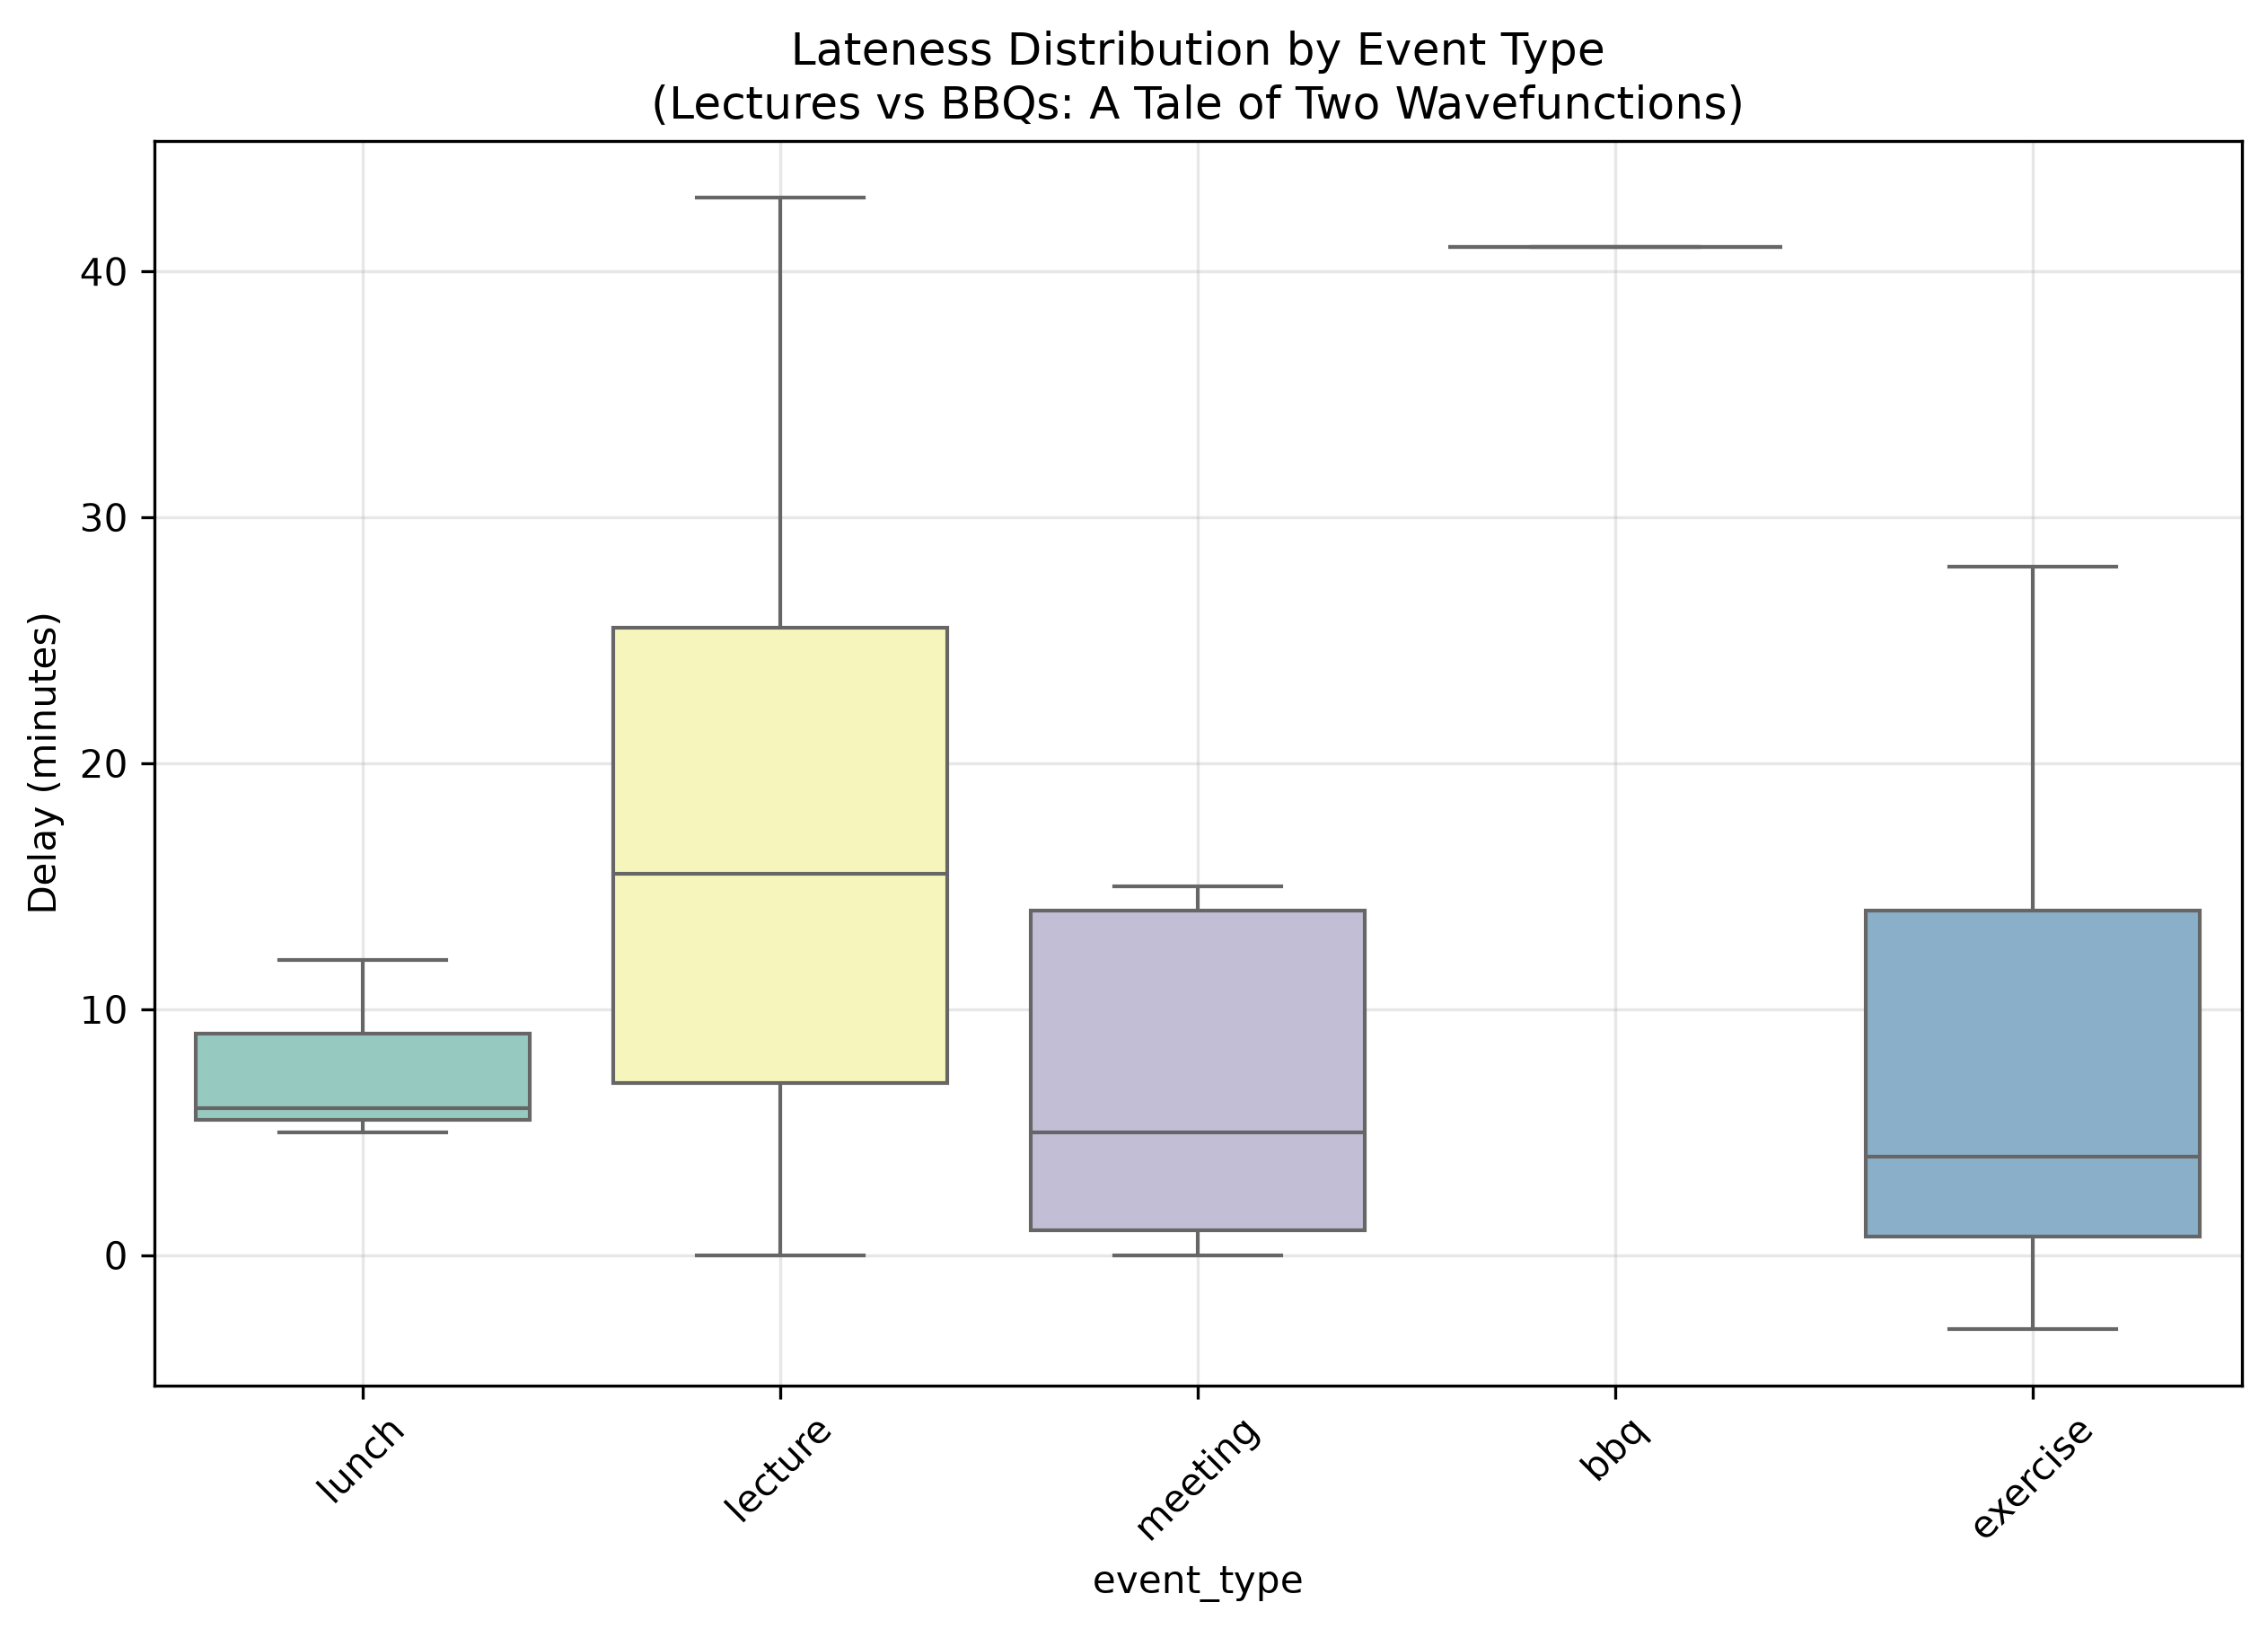
\includegraphics[width=\linewidth]{../plots/boxplot_by_event.png}
    \caption{
        Delay distributions by event type.
        Lectures occupy a strongly coupled phase; meetings
        and exercises are closer to the Gaussian fixed
        point. The barbecue is no longer the unique
        infrared catastrophe.
    }
    \label{fig:box}
\end{figure}

\begin{table}[H]
\centering
\caption{Delay statistics by event type (attended events).}
\label{tab:event}
\small
\begin{tabular}{lcccc}
\toprule
Event & $n$ & Mean & Median & Max \\
\midrule
Lecture  & 18 & 17.8 & 15.5 & 43 \\
Exercise & 12 &  8.3 &  4.0 & 28 \\
Meeting  &  5 &  7.0 &  5.0 & 15 \\
Lunch    &  3 &  7.7 &  6.0 & 12 \\
BBQ      &  1 & 41.0 & 41.0 & 41 \\
\bottomrule
\end{tabular}
\end{table}

\subsection{Time-of-day and Weekday Dependence}

Scheduled hour is not a spectator variable. Events at 12:15
--- the functional-analysis lecture slot --- have mean delay
$27.7$~min ($n=6$). Friday 16:15 Mathematica exercises
have mean $5.2$~min ($n=9$) and contain two of the
on-time arrivals. The 08:30 exercise slot is bimodal:
one early arrival and two delays of $27$--$28$~min,
with a majority of the remaining slots lost to absence.

Weekdays tell the same story in a different basis. Tuesday
(mean $25.4$~min) and Thursday (mean $17.6$~min)
host the functional-analysis lectures and remain the late
sector. Friday (mean $5.2$~min, median $4$~min) is the
closest approximation to an ordered phase. Monday is
intermediate ($10.9$~min) and mixes Mathematica lectures
with project meetings.

A minimal effective description is therefore
\begin{equation}
    \langle\Delta t\rangle
    =
    \Delta t_0
    + g_{\mathrm{FA}}\,\mathcal{O}_{\mathrm{FA}}
    + g_{12}\,\mathcal{O}_{12:15}
    + \cdots
\end{equation}
Here $\Delta t_0$ is a baseline mean delay;
$\mathcal{O}_{\mathrm{FA}},\mathcal{O}_{12:15}\in\{0,1\}$ 
are indicators for functional analysis and the
noon slot; and $g_{\mathrm{FA}}$, $g_{12}$ are the
associated couplings in minutes.
The two operators are almost collinear in this timetable,
so subject and clock time cannot yet be separated.

\subsection{Survival Analysis}

Treating arrival as a decay process, we define the empirical
survival function among attendees,
\begin{equation}
    S(t) = P(\Delta t > t).
\end{equation}
The measured values decay roughly exponentially:
\begin{center}
\small
\begin{tabular}{lccccc}
\toprule
$t$ (min) & 0 & 10 & 20 & 30 & 40 \\
$S(t)$ & 0.85 & 0.51 & 0.26 & 0.10 & 0.05 \\
\bottomrule
\end{tabular}
\end{center}
After twenty minutes, one quarter of the attended sample
has still not arrived; after forty minutes the survival
probability has dropped to two events (the barbecue and
the $43$~min lecture). If no-shows were interpreted as
$\Delta t=\infty$, $S(t)$ would approach
$P_{\mathrm{absent}}\simeq 0.36$ rather than zero --- a
finite late-time vacuum persistence, now larger than in
the first observing season.

\subsection{Weather Correlation and Cultural Prior Effects}

We test for correlations between meteorological conditions and
arrival-time residuals, in particular:
\begin{itemize}[leftmargin=0.4cm]
    \item precipitation vs.\ lateness,
    \item temperature vs.\ lateness.
\end{itemize}

A naive hypothesis suggests that adverse weather conditions
(e.g.\ rain) should increase delays due to reduced mobility and
lowered external efficiency.

However, the observed data exhibit a counterintuitive trend:
rainy conditions are weakly associated with improved punctuality.

The Pearson correlation between temperature and delay remains
consistent with zero ($r\simeq -0.02$). Sunny attendances
average $15.0$~min and include the barbecue;
cloudy attendances average $12.5$~min. The only
properly rainy attendance is still the unique early arrival
($\Delta t=-3$~min at $9^{\circ}\mathrm{C}$ on 6~May 2026).
Drizzle is not similarly virtuous: it coincides with a
$38$~min lecture delay and one exercise no-show.
Precipitation, if it is a coupling at all, is therefore not
a monotonic one.

One possible interpretation is a cultural prior effect: in
populations with high familiarity with rainy conditions, such as
central European subjects, precipitation may not constitute a
significant perturbation to scheduling dynamics.

More speculatively, one may hypothesize a \textit{rain-resonance effect},
where meteorological stress aligns with reduced dispersion in
temporal decision-making, effectively collapsing the motivational
wavefunction into a more localized arrival-time distribution.

Figure~\ref{fig:weather} summarizes the temperature--delay plane,
colored by weather. We stress that this interpretation remains
highly conjectural and requires significantly larger datasets
for validation. In particular, the rain-resonance claim is
currently supported by a single point and should be regarded
as a target for a dedicated follow-up run, preferably in
November.

\begin{figure}[H]
    \centering
    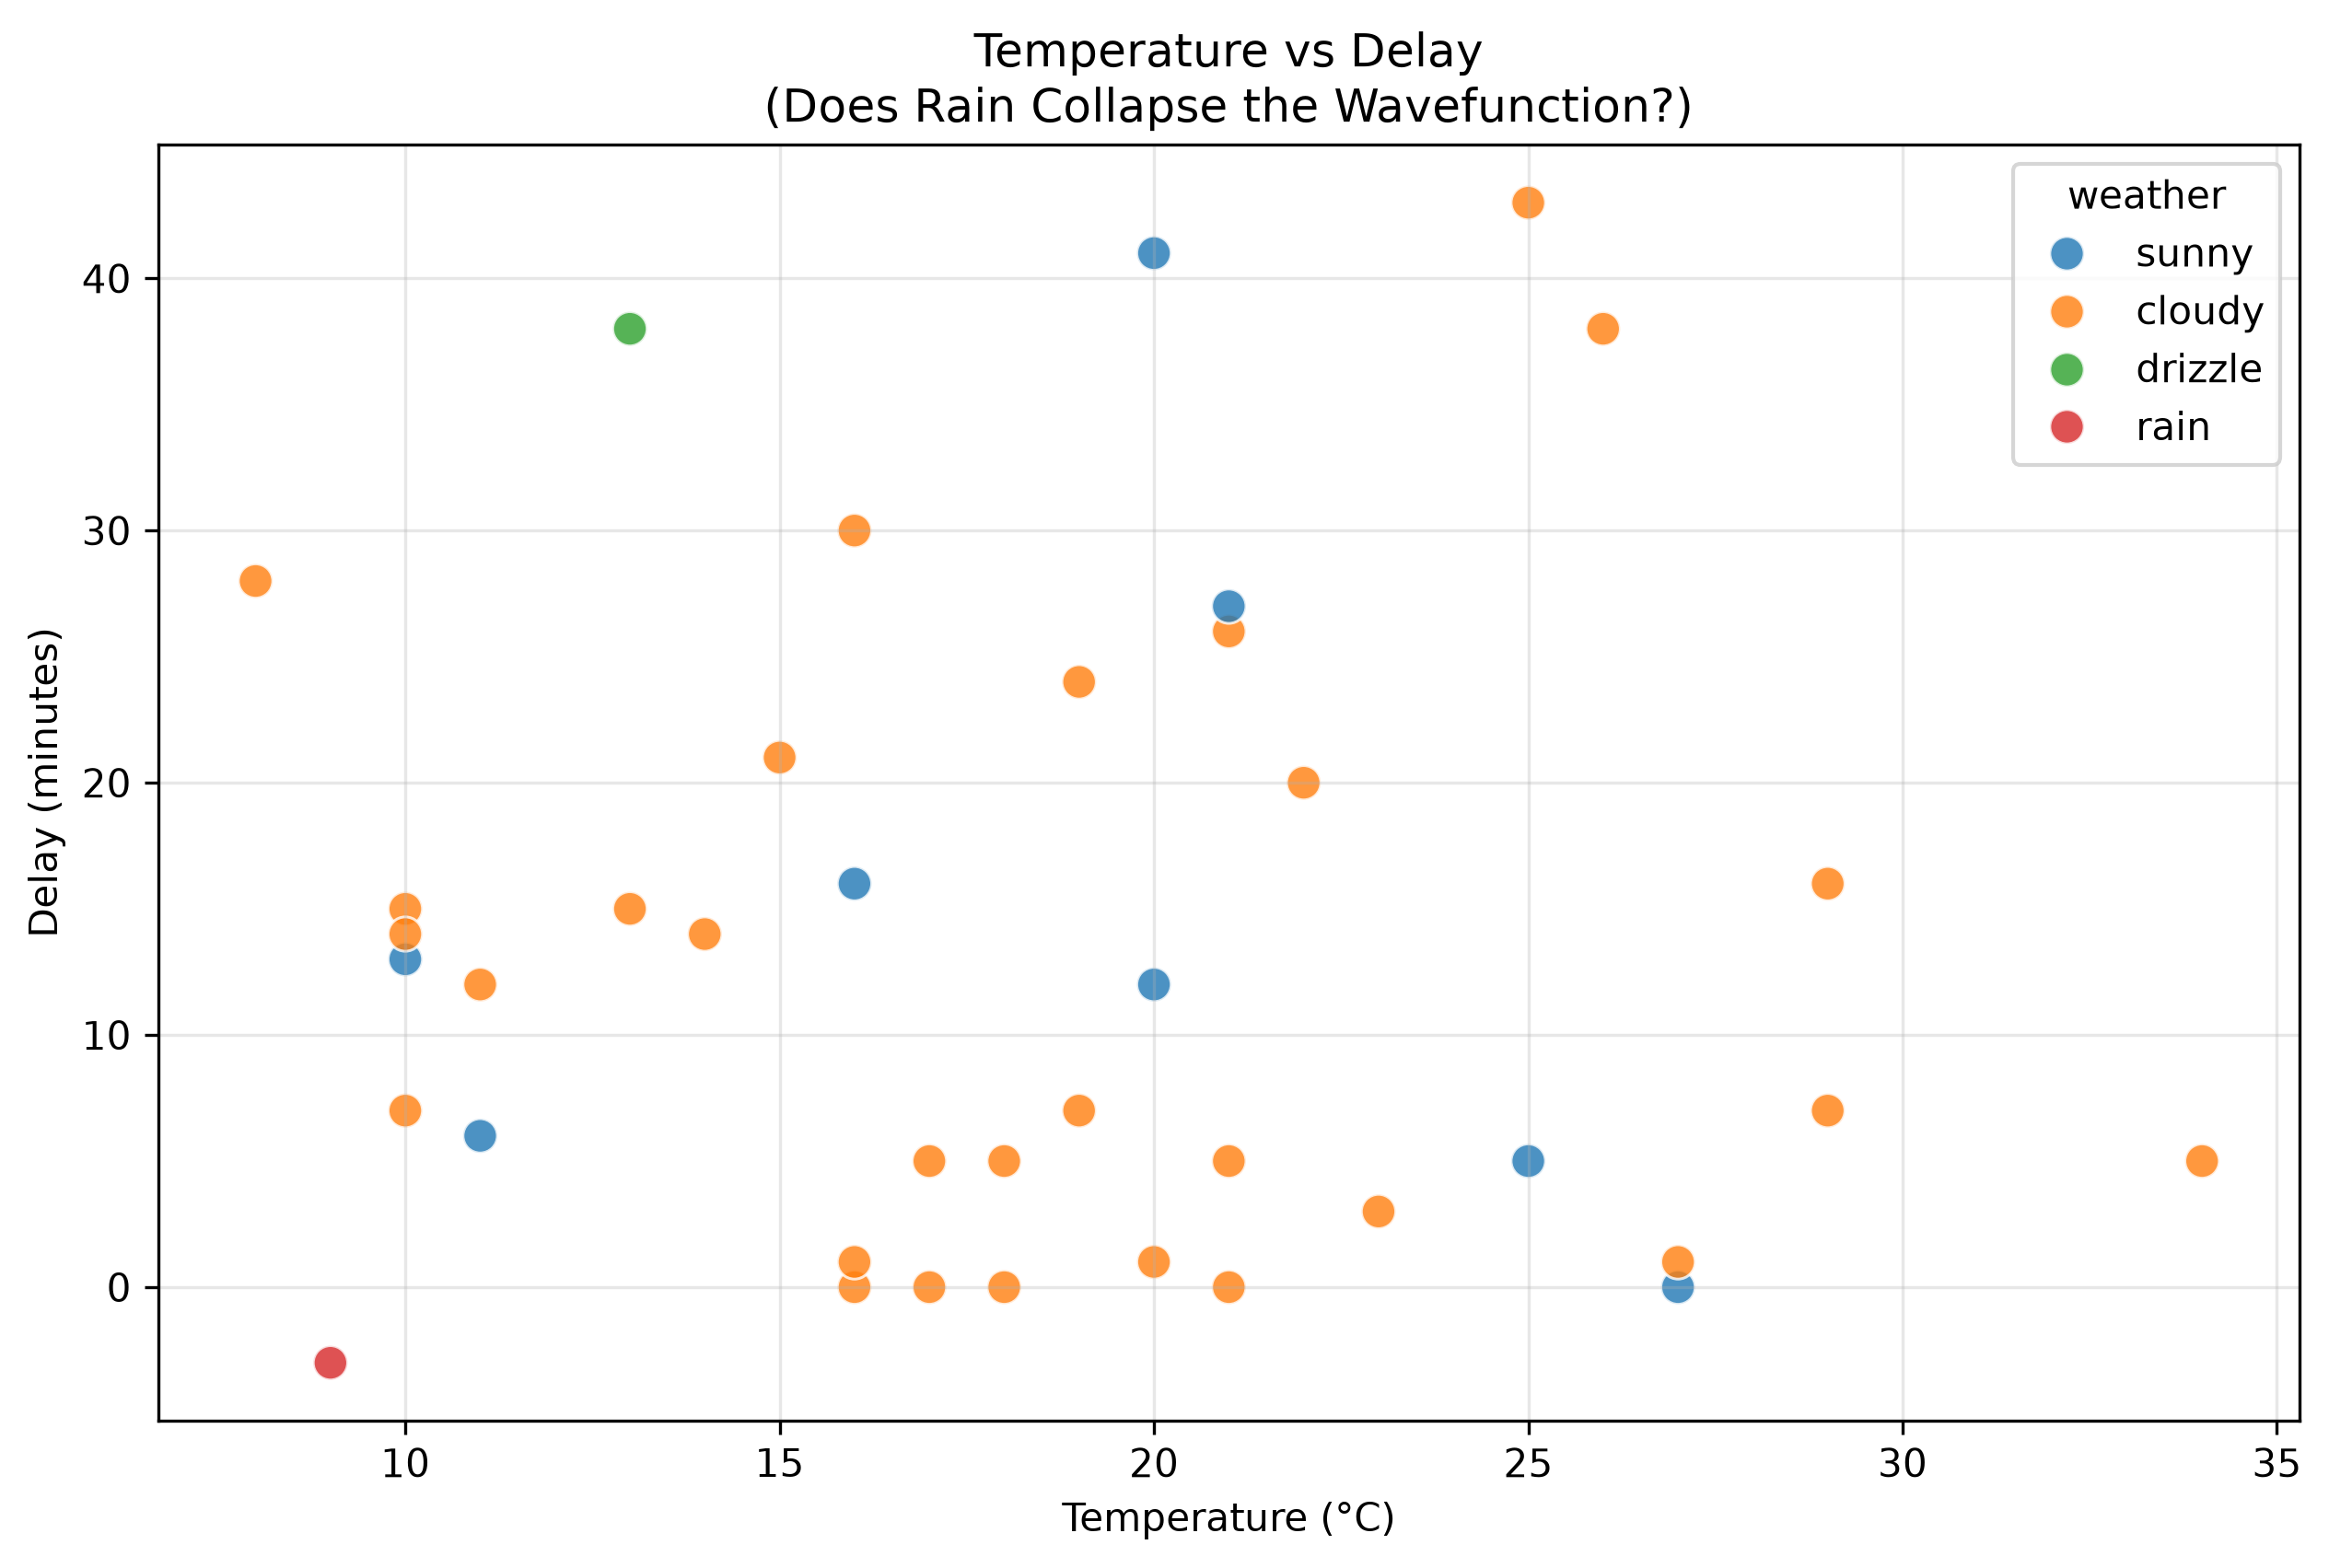
\includegraphics[width=\linewidth]{../plots/weather_scatter.png}
    \caption{
        Delay versus ambient temperature, colored by weather.
        No linear thermal trend is visible.
        The isolated red point is the early-arrival rain
        event; the isolated green point is the
        $38$~min drizzle lecture.
        Whether rain collapses the wavefunction, or merely
        failed to prevent one on-time morning, cannot be
        decided from this sample.
    }
    \label{fig:weather}
\end{figure}

% -------------------------------------------------
\section{A Phenomenological Model}
% -------------------------------------------------

The data motivate a minimal two-phase description.
Let $p_0$ be the probability of remaining in the punctuality
vacuum (the empirical rate $P(\Delta t\le 0)\simeq 0.15$)
and $1-p_0$ the probability of tunneling into the late
continuum. Write
\begin{equation}
    \Delta t
    =
    \begin{cases}
      \varepsilon, & \text{with probability } p_0, \\[2pt]
      \Delta t_{\min} + \tau\,\xi, & \text{otherwise}.
    \end{cases}
\end{equation}
Here $\varepsilon$ is a narrow random variable supported
near zero (in the sample, $\varepsilon\in\{-3,0\}$);
$\Delta t_{\min}>0$ is a small offset for the onset of
the late phase;
$\tau\simeq 15$~min is the exponential scale fitted to
positive delays;
and $\xi\sim\mathrm{Exp}(1)$ is a unit exponential random
variable, i.e.\ it has density $e^{-x}$ for $x>0$ and
mean $1$. The product $\tau\xi$ is therefore an
exponential delay with mean $\tau$.

An equivalent field-theoretic cartoon is an asymmetric
effective potential $V(\Delta t)$ with a shallow well at
$\Delta t=0$ and a linear downhill slope for $\Delta t>0$.
Once the well is left, there is no classical restoring
force; arrival becomes a first-passage problem with
constant hazard $1/\tau$.

Reminders, if they were applied, could be added
perturbatively. Let $R$ denote a reminder strength
(for example a dimensionless count of messages, or an
intensity in inverse minutes) and let $\alpha$ be the
associated linear coupling, with expected sign
$\alpha<0$. Then
\begin{equation}
    \Delta t
    =
    \Delta t_0 + \alpha R + \mathcal{O}(R^2),
\end{equation}
where $\Delta t_0$ is the delay in the absence of
reminders. No controlled reminder protocol was implemented
in this run, so $\alpha$ is not measured.

The event-type dependence is encoded by letting the tail
scale run with the appointment,
\begin{equation}
    \tau
    =
    \tau_0
    + c_{\mathrm{FA}}\,\mathcal{O}_{\mathrm{FA}}
    + c_{\mathrm{BBQ}}\,\mathcal{O}_{\mathrm{BBQ}}.
\end{equation}
Here $\tau_0$ is a baseline scale,
$\mathcal{O}_{\mathrm{FA}},\mathcal{O}_{\mathrm{BBQ}}\in\{0,1\}$
are indicator functions for functional-analysis lectures
and barbecues, and $c_{\mathrm{FA}}$, $c_{\mathrm{BBQ}}$
are the corresponding shifts in $\tau$, in minutes.
Fits of this form are underconstrained, yet the hierarchy
$\tau_{\mathrm{FA}} > \tau_{\mathrm{lecture}}
> \tau_{\mathrm{meeting}} \sim \tau_{\mathrm{exercise}}$
is already visible in Table~\ref{tab:event}. In
renormalization-group language, functional analysis is a
relevant deformation of the punctuality fixed point;
Friday Mathematica exercises are closer to the trivial
(on-time) theory.

A crude Bayesian forecast for a new event of type $s$ is
the posterior predictive implied by the corresponding
subsample. For a noon functional-analysis lecture one
should budget $\langle\Delta t\rangle\simeq 28$~min
and keep a heavy tail in mind. For a Friday exercise the
prior is kinder.

% -------------------------------------------------
\section{Discussion}
% -------------------------------------------------

Several features of the data suggest scale-dependent
punctuality dynamics rather than Gaussian noise around a
well-intentioned schedule.

Small delays ($\Delta t\lesssim 5$~min) are compatible
with ordinary transit fluctuations and with the five recorded
on-time events. They form the metastable vacuum of the model
above. Delays exceeding $20$~min --- ten events --- occupy a
strongly coupled regime in which additional waiting time is
cheap. The exponential tail is the quantitative expression of
that cheapness, and its scale has been stable across the two
observing seasons.

The rare early-arrival event of 6~May 2026
($\Delta t=-3$~min, rain, 08:30 exercise) remains unique
after five additional weeks. It may represent either a
statistical fluctuation or evidence of spontaneous
punctuality symmetry breaking. We cannot distinguish these
possibilities. We note only that it occurred in the one
environment that a naive mobility model would have predicted
to be \emph{worse}, which is either a joke played by a small
sample or a genuine rain-resonance.

Two negative results are worth stating clearly.
Temperature does not correlate with delay, so a simple
thermal-activation picture of getting out of bed is not
supported at the level of ambient Celsius.
And social context does not automatically restore order:
the barbecue is no longer the largest residual, but it
is still not an ordered phase.

The no-show channel deserves to be treated as physics rather
than as missing data. At $36\%$, it is the dominant
inefficiency of the experiment. Field notes list workshop
clashes, back pain, laboratory conflicts, presentation
practice, oversleeping, and a Berlin trip --- a
heterogeneous set of ultraviolet completions that all flow
to the same infrared observable (the empty chair).
A future analysis could model attendance as a binary field
coupled to $\Delta t$, with correlated late and absent
phases. The functional-analysis sector already looks like
a joint late/absent phase.

Limitations are obvious and mostly statistical.
The catalog spans fourteen weeks, not a thermodynamic limit.
Several weather and event-type bins have $n=1$.
Subject and time of day remain confounded by the lecture
timetable. Two Berlin days are a known detector-off period.
The observer is not independent of the subject in the social
sense, even though the subject was not informed.
None of these caveats removes the central phenomenological
fact: a working theoretical physicist can be assigned a
delay scale of a quarter of an hour, a punctuality rate of
one in seven attendances, and a better-than-even chance of
not appearing at a functional-analysis lecture.

% -------------------------------------------------
\section{Conclusion}
% -------------------------------------------------

We have presented a statistical characterization of
arrival-time behavior in a single theoretical-physicist
subject over 61 scheduled events.

The data reject a symmetric Gaussian model of punctuality.
The attended delay distribution is positively skewed, has
mean $13.3$~min and median $12$~min, and is consistent
with an exponential tail of scale $\tau\simeq 15$~min.
Strict punctuality occurs in $15\%$ of attendances.
An additional $36\%$ of scheduled events are no-shows,
so the joint probability of presence and non-lateness is
$10\%$.

The lateness coupling runs with academic context.
Functional-analysis lectures at noon are the strongly
coupled sector, now including the $43$~min global record.
Friday Mathematica exercises and project meetings remain
closer to a perturbative phase.
Weather does not act as a simple mobility friction;
the only early arrival still occurred in the rain.

A two-phase phenomenological model --- a shallow
punctuality well plus a memoryless late continuum ---
organizes these facts without overclaiming
microscopic mechanism. Additional data, a controlled
reminder coupling, and an independent autumn-rain run
will be required to decide whether a stable punctuality
phase can ever be reached under laboratory conditions.

% -------------------------------------------------
\section{Outlook}
% -------------------------------------------------

The present work has been largely phenomenological: a catalogue of
arrival-time residuals, a two-phase effective description, and a
running lateness coupling whose strongest deformation is functional
analysis. A fundamental model capable of \emph{deriving} these
patterns from microscopic motivational dynamics remains to be
constructed. No connection to gravitational theory is expected, but
it cannot be ruled out at the present stage of the research programme.

Equally incomplete is the experimental side. The sample is still a
single-subject run. Comparable data on distinguishable sets of
theoretical physicists have not yet been produced, and a formal
definition of \textit{theoretical physicist} suitable for multi-subject
statistics is still lacking. Until both the microscopic theory and
the multi-subject control sample exist, the results reported here
should be regarded as a carefully measured correlation function of
one friend, not as a universal law of academic time.

Further remarks, data, and contributions on the present research
subject are cordially invited and may be communicated to
\texttt{mhuang@ep1.rub.de}.

% -------------------------------------------------
\section*{Acknowledgments}
% -------------------------------------------------

The author acknowledges useful discussions with the subject,
who remained unaware of the ongoing experiment throughout the
entire data acquisition phase, and with the second observer
Simon, who appears to be a relevant operator in his own right.
This manuscript is intended as a birthday observable:
a complete, if slightly unflattering, correlation function
of a friend.

% -------------------------------------------------
\section*{Funding Statement}
% -------------------------------------------------

This research received no governmental or institutional funding. Applications for support from the European Research Council (ERC), the U.S. National Science Foundation (NSF), and the Deutsche Forschungsgemeinschaft (DFG) are currently pending. The work was funded exclusively by private donations from individuals of Chinese background.

We thank the Institute of Physics and Astronomy at Ruhr-Universität Bochum for providing institutional support and research facilities that facilitated this work.

\end{document}